\section{Significance of Project}

Core-collapse supernovae (CCSNe) are the most extreme laboratories for nuclear physics in the universe.
Stellar core collapse and the violent explosions that follow give birth to neutron stars and black holes, and in the process synthesize most of the elements heavier than helium throughout the universe.
The behavior of matter at supranuclear densities is crucial to the CCSN mechanism, as are strong and weak interactions.
Beyond Standard Model behavior of neutrinos may also impact the CCSN mechanism.
Despite the key role CCSNe play in many aspects of astrophysics, and decades of research effort, {\it we still do not fully understand the details of the physical mechanism that causes these explosions.}
This leaves frustratingly large error bars on many key aspects of our theoretical understanding of the universe, and also makes it difficult to constrain uncertain nuclear physics with data from CCSNe.

We propose an end-to-end, multi-year investigation of CCSNe that includes the effects of rotation, magnetic fields, and progenitor asphericity.
Our comprehensive research program will consist of 3D MHD CCSN simulations with sophisticated multi-dimensional neutrino transport, the most realistic initial conditions ever adopted for the study of CCSNe, and an intensive comparison to observations through the calculation of gravitational wave emission, detailed nucleosynthesis, and electromagnetic radiative transfer.
The ambitious objectives of this project will be achievable by leveraging the unique combination of skills in the proposal team, cutting-edge open-source software, and the Leadership-class resources available through the INCITE program.

\subsection{Achievements with Previous INCITE Allocation}
\label{sec:achievements}

The PI is also PI of the 2015-2017 INCITE allocation ``Petascale Simulation of Magnetorotational Core-collapse Supernovae.''
Based on simulations performed during Year 1 of that project, we have shown that modest rotation and magnetic fields can have a signficant impact on the CCSN mechanism, both acting to lower the threshold to explosion in 3D.
Additionally, using extremely high-resolution simulations of MHD turbulence in the CCSN gain region carried out as part of that project, we demonstrated that the gain region is also unstable to growth of the magnetorotational instability (MRI), implying exponential growth of magnetic field strengths and potential important impact on the rate of turbulent dissipation \citep[e.g.,][]{Thompson:2005}.
Regions of MRI growth in the entire post-shock region are shown in the left panel of Figure \ref{fig:incite2015}.

During Year 2 of that INCITE project, we carried out high-resolution 3D simulations of CCSNe with multidimensional M1 neutrino transport.
These simulations have shown the presence of the standing accretion shock instability (SASI) and have shown that progenitor perturbations can aid shock expansion (middle panel of Figure \ref{fig:incite2015}).
By 500 ms, however, we have yet to see the initiation of an explosion in any of our models.
A few of the most promising cases are being continued to later times at present.

During Year 3 of the previous INCITE allocation, we are running 3D MHD CCSN simulations including M1 neutrino transport.
These simulations are just now getting underway but will serve as crucial pre-cursors to the simulations we plan in the present proposal.

Several publications on the results of our simulations from the previous INCITE allocation are currently in preparation or already under review.

\begin{figure}
  \centering
  \begin{tabular}{lll}
    \includegraphics[width=1.5in]{figs/o110b9_C90_0566} &
    \includegraphics[width=3in]{figs/mesa20vsPert} &
    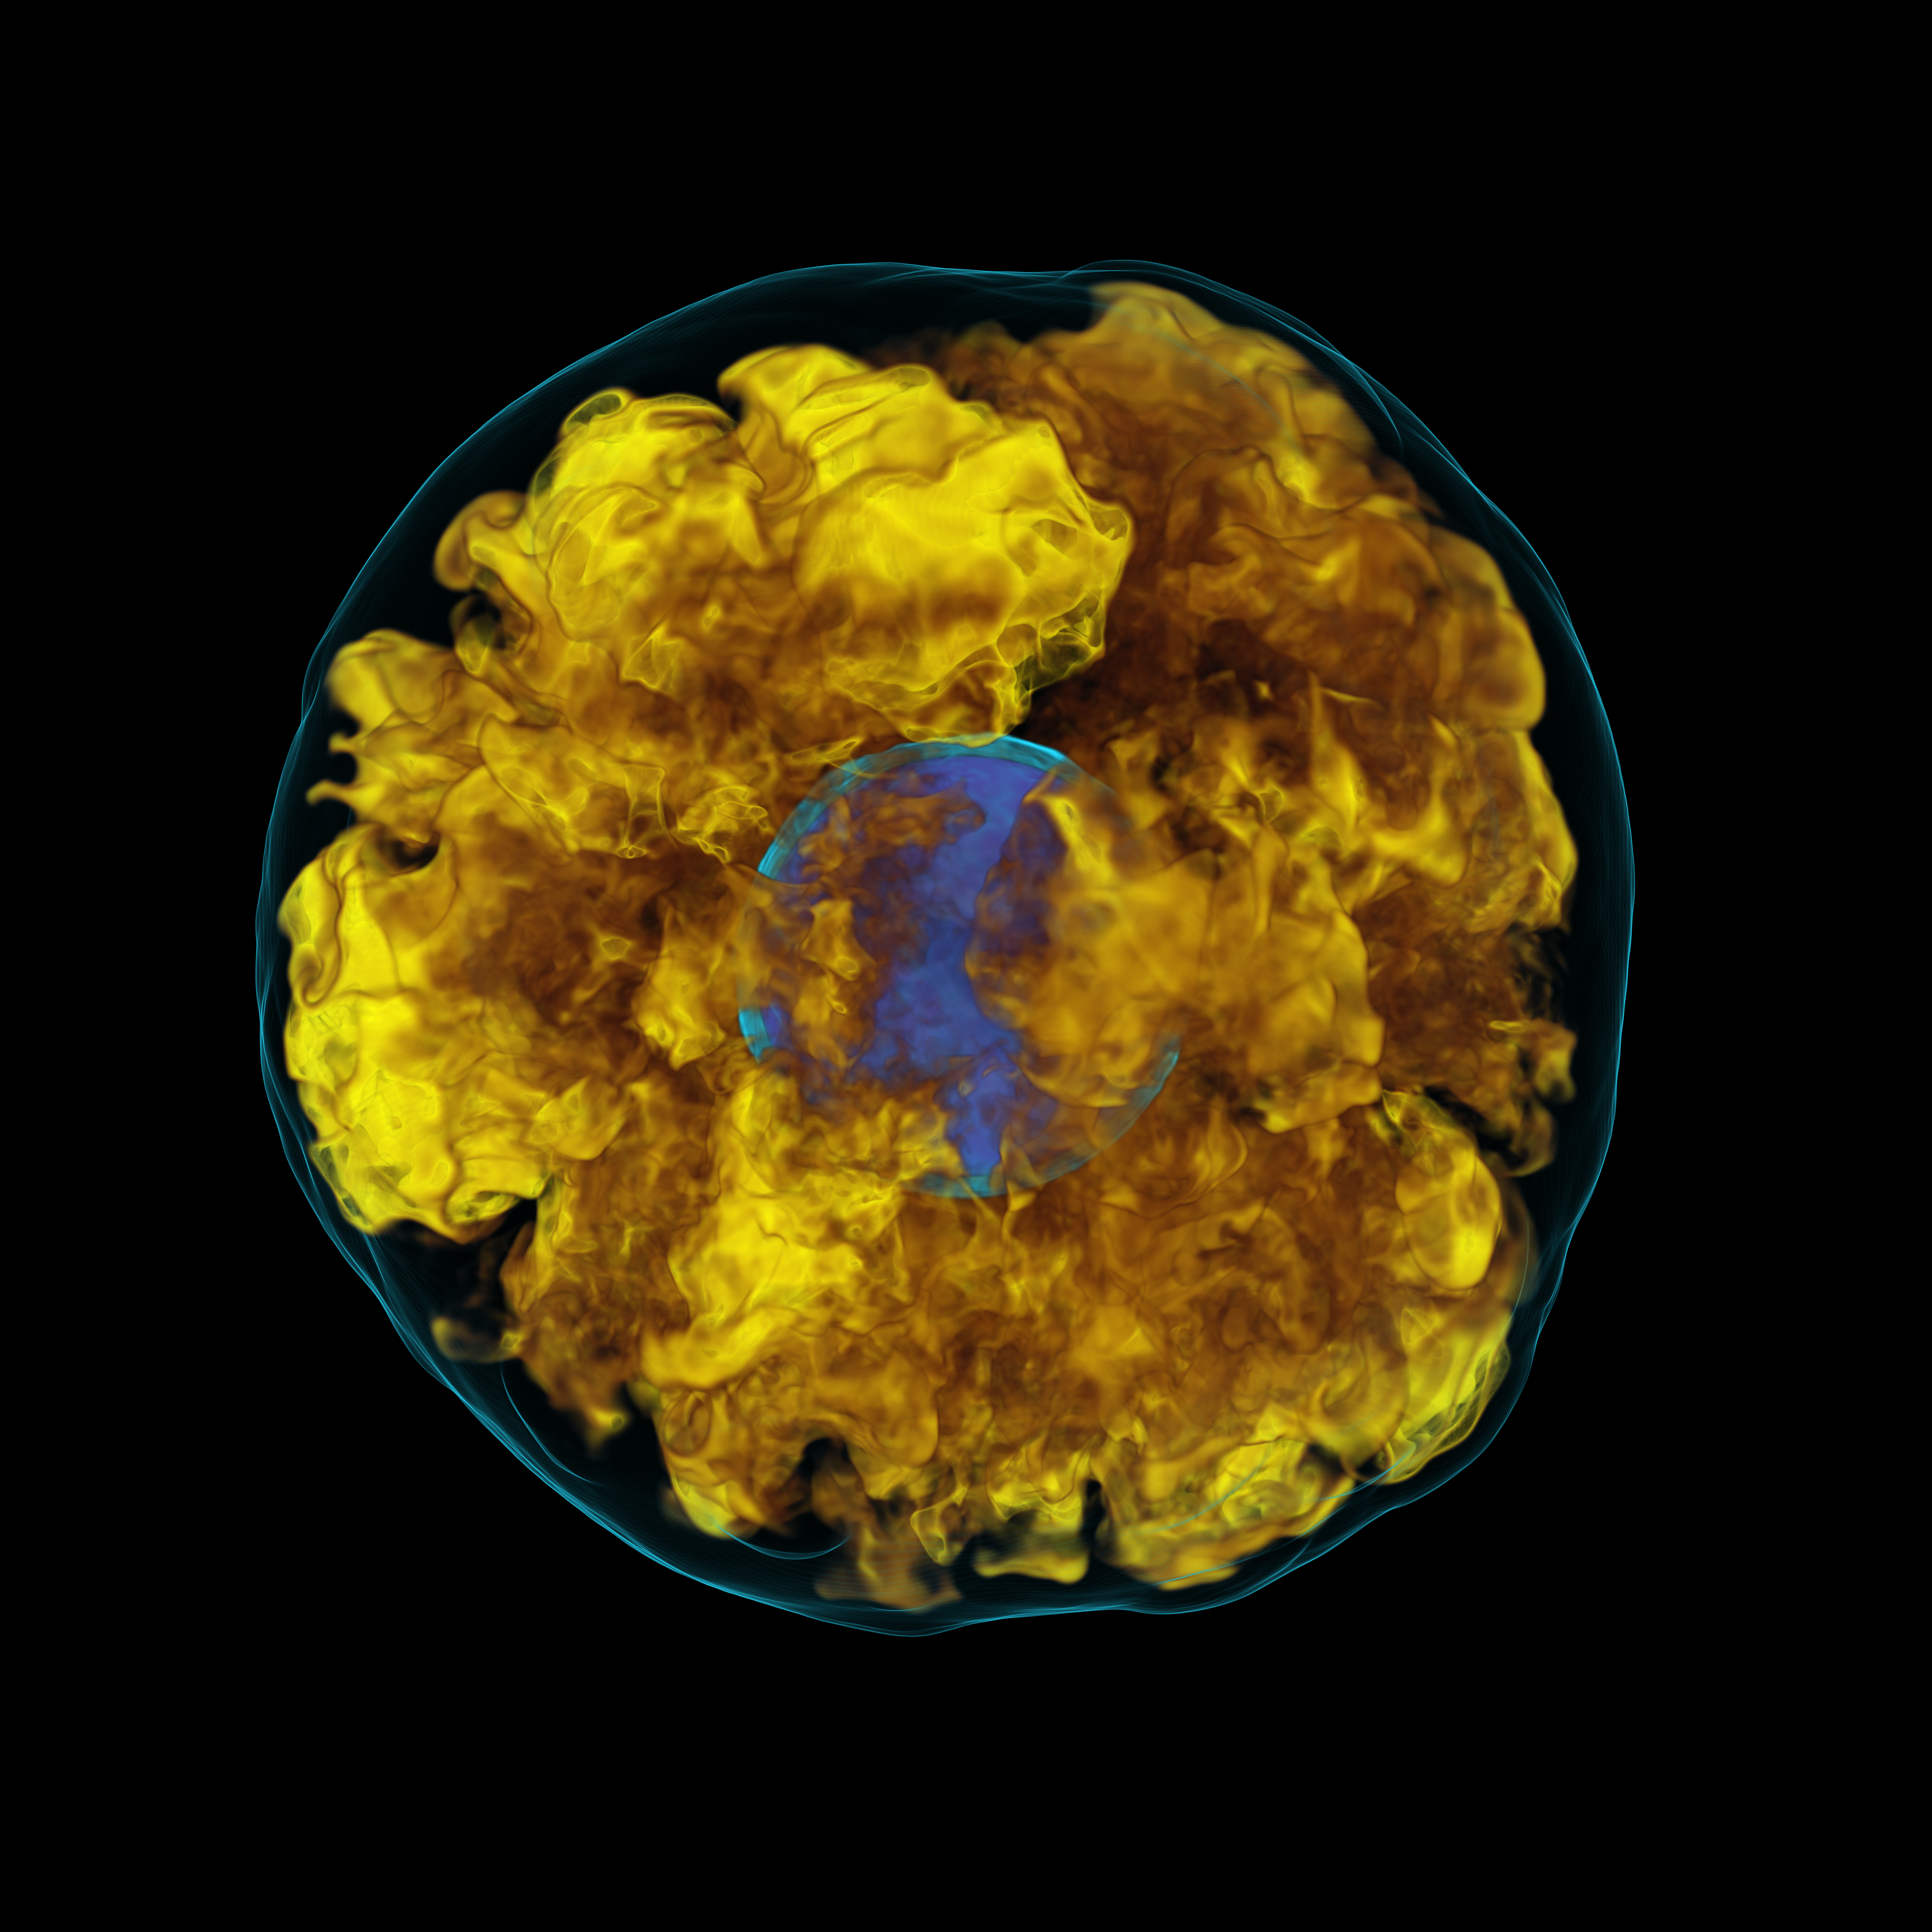
\includegraphics[width=1.5in]{figs/fig_vr_mesa20_pert_0232_v2}
  \end{tabular}
  \caption{{\bf Left:} Regions of instability to the MRI in a 3D CCSN simulation. Blue regions indicating growth of the MRI. {\bf Center:} Results for 3D M1 neutrino tranport simulations in a 20-\msun star. {\bf Right:} Volume rendering of entropy from a 3D CCSN simuulations with M1 neutrino transport.}
  \label{fig:incite2015}
\end{figure}

\subsection{Background}

Despite over a half-century of theoretical and computational effort, the detailed nature of the mechanism that reverses stellar core collapse and drives robust CCSN explosions remains uncertain.
In the final stages of nuclear burning, massive stars form inert iron cores.
These iron cores grow via silicon shell burning to beyond their maximum stable mass, the effective Chandrasekhar limit, at which point gravitational collapse ensues.
This collapse is accelerated by ever-increasing neutrino cooling, photodissociation of iron nuclei, and electron captures onto protons.
The collapse proceeds until the central regions of the core exceed nuclear density.
At such small inter-nucleon spacings, the strong nuclear force becomes repulsive and dramatically halts the collapse.
This effective stiffening of the equation of state launches a strong shock wave into the still collapsing outer part of iron core.
Early calculations of this process in spherical symmetry suggested that this ``bounce'' shock would be sufficiently energetic to unbind the outer parts of the collapsing star and power the supernova explosion \citep{Colgate:1961}.
But it was quickly realized that catastrophic neutrino cooling behind the shock and photodissociation of the infall iron nuclei by the shock would lead to an enormous amount of energy loss causing the shock to stall.




%
% The last few years have seen the advent of 3D simulations with high-fidelity treatments of the input physics \citep[e.g.,][]{Hanke:2013, Tamborra:2014, Melson:2015, Melson:2015a, Lentz:2015, Janka:2016}.
% 3D simulations including high-fidelity parameter-free treatments of energy-dependent neutrino transport are extremely challenging and expensive, requiring on the order of 100 million core-hours on current Leadership-class supercomputers {\it per simulation}.
% Complimenting these ``full-physics'' simulations, many 3D simulations of the CCSN mechanism have been carried out using approximate treatments of the neutrino physics in order to drastically reduce the computational expense \citep[e.g.,][]{Nordhaus:2010, Hanke:2012, Burrows:2012, Couch:2013a, Murphy:2013, Dolence:2013, Couch:2013b, Iwakami:2014, Couch:2014, Couch:2015}.
% These studies are often targeted at addressing specific questions for which the approximations made are appropriate.
%
% One of the first and most important questions addressed in this way was: Are explosions obtained more easily in 3D than in 2D?  In other words, is 3D the missing key to robust supernova explosions across the broad range of progenitor masses?
% Using a ``lightbulb'' treatment for the neutrino heating and cooling, wherein the neutrino luminosity emerging from the proto-neutron star is set by hand \citep{Murphy:2008}, \citet{Nordhaus:2010} found that explosions were obtained significantly more easily in 3D than in 2D.
% Using a very similar approach, \citet{Hanke:2012} were unable to reproduce this result, finding instead significant stochasticity and resolution-dependence.
% Having fixed an issue with their gravity solver, \citet{Dolence:2013} update the results of \citet{Nordhaus:2010} and find dramatically smaller differences between the likelihood for explosion between 2D and 3D, though their results still favored explosions in 3D over 2D.
% We also carried out a comparison between 2D and 3D using the lightbulb approximation in FLASH \citep{Fryxell:2000, Dubey:2008}, which we had for the first time adapted to treat the microphysics of the CCSN mechanism \citep{Couch:2013a}.
% With high-resolution simulations, we found that 3D simulations were {\it less} prone to explosion that comparable 2D simulations.
% Confirming the suspicions of \citet{Hanke:2012}, we showed that this is due largely to artificial behavior in 2D, namely the exaggeration of the growth of the SASI and the inverse turbulent cascase which transports turbulent energy to large scales rather than to small scales as is the case in 3D.
%
% The implication that successful explosions in 2D may not translate to 3D demanded verification with better input physics.
% We carried out a very detailed comparison of 2D and 3D CCSN simulations in two different progenitor star models \citep{Couch:2014}.
% Our results confirmed the earlier lightbulb results of \citet{Hanke:2012, Couch:2013a}: 2D simulations exploded more readily than 3D.
% Crucially, this is due essentially to numerical artifacts that result from the forced axisymmetry of 2D simulations.
% Around the time we presented our work in \citet{Couch:2014}, other groups using parameter-free treatments for the neutrino transport showed similar results: all else being equal, 2D simulations exploded more easily than 3D \citep{Hanke:2013, Tamborra:2014, Takiwaki:2014}.
% And the 3D simulations with the most accurate neutrino transport and physics \citep{Hanke:2013, Tamborra:2014} failed to find 3D explosions at all for progenitor models that exploded in 2D.
%
% Fortunately, this bleak situation has not entirely persisted.
% There are now in the literature a handful of cases showing successful neutrino-driven explosions in 3D full-physics simulations \citep{Melson:2015, Melson:2015a, Lentz:2015}.
% One of these is for a low-mass progenitor which also explodes in 1D simulations \citep{Melson:2015}.
% In another, an explosion was driven in a 20 $M_\odot$ star by a modified neutrino-nucleon scattering cross sections that {\it might} be expected if strange-quarks play an important role \citep{Melson:2015a}.
% For the 15 $M_\odot$ progenitor of \citet{Woosley:2007d}, \citet{Lentz:2015} report a successful explosion in 3D, though the explosion sets in later than the comparable 2D simulation and the explosion energy is smaller.
% Thus, there are encouraging full-physics results in 3D, although 3D simulations do seem to be less favorable for explosion than 2D.
%
%
% Another potential issue with current 3D simulations is that the tremendous expense of the neutrino transport necessitates the use of low resolution, typically about $2^\circ$ in the spherical angular dimensions with comparable radial spacing.
% Low resolution is concerning because much recent work has pointed out the importance of turbulence in the CCSN mechanism \citep{Murphy:2011a, Hanke:2012, Couch:2013a, Murphy:2013, Couch:2013b, Couch:2015, Melson:2015a, Couch:2015a, Abdikamalov:2015, Radice:2015a}, and turbulence is notoriously difficult to adequately resolve in numerical simulations.
% In the context of the CCSN mechanism turbulence exerts an effective dynamic pressure that can help to hold up the shock against the ram pressure of the infalling core of the progenitor star \citep{Murphy:2013}.
% We showed that under a broad range of conditions this turbulent pressure can be as large of 40-50\% of the background thermal pressure in the gain region behind the stalled shock \citep{Couch:2015}.
% This is an order-unity effect in understanding the stability of the shock.
% We also directly connected the presence of non-spherical motion in the progenitor star with stronger post-shock turbulence and higher likelihood for explosion \citep{Couch:2013b}.
% We went on to show that such strong, large-scale non-spherical motion is an unavoidable outcome of nuclear burning in the final stages of evolution of a massive star \citep{Couch:2015a}.
% This work entailed the first ever 3D simulation of the final minutes in the life of a massive star up to and including the self-consistent onset of gravitational instability and core collapse.
%
% The elephant in the room with respect to turbulence in the CCSN mechanism is the challenge of accurately capturing its behavior at finite resolution.
% Many multidimensional studies have reported resolution dependence in the CCSN mechanism \citep[e.g.,][]{Hanke:2012, Couch:2013, Couch:2014, Takiwaki:2014, Abdikamalov:2015}, but in \citet*{Radice:2015} we set out to conduct a controlled numerical experiment to address what resolution was {\it needed} to accurately capture the behavior of turbulence in the CCSN context.
% Turbulent media are often characterized by the Reynolds number, the ratio of inertial to viscous forces, with more turbulent systems having larger Reynolds numbers.
% The medium behind the stalled supernova shock is highly inviscid, yielding enormous Reynolds numbers of order $10^{17}$ \citep{Abdikamalov:2015}.
% The trouble is that with the numerical methods used to study CCSNe, the Reynolds numbers in the simulations are set by numerical effects arising from finite grid resolution.
% Even the current highest resolution simulations have numerical Reynolds numbers estimated to be {\it less than a few hundred} \citep{Couch:2015, Abdikamalov:2015}.


The over-arching goal of the theoretical investigation of the CCSN mechanism is to make {\it explanatory} and {\it predictive} connection to observation and experiment.
Doing this in a rigorous way requires a successful, physically accurate model for the explosion mechanism.
Even studies of stellar nucleosynthesis from massive stars \citep[e.g.,][]{Woosley:1995, Woosley:2007d}, which arguably only require that an energetic explosion occur in massive stars, are limited to studying only low mass nuclei since the high mass nuclei can only be synthesized deep within the explosion where the details of the mechanism play a crucial role.
Any investigation of high-mass element formation (i.e., the r-process) in CCSNe requires a self-consistent model for the explosion mechanism.
This is a critical need for connecting nuclear astrophysics to current and future experimental efforts at, e.g., JLAB, RHIC, NSCL, FRIB, etc.
Armed with \nth{21}-century tools, the solution to this problem that has been vexing us since the \nth{20} century may finally be within reach.
Successful, energetic explosions across an adequate range of progenitor star masses may hinge on 3D hydrodynamics that captures the correct behavior of turbulence, general relativistic gravity, accurate energy-dependent neutrino transport, sophisticated microphysics based on modern nuclear theory, and realistic stellar progenitor models that directly model the truly 3D structure of massive stars \citep[e.g.,][]{Meakin:2007, Arnett:2011, Couch:2015a}.


%%% NEW

All stars rotate and have magnetic fields.
Following massive star core collapse, rapid rotation and strong magnetic fields can lead to powerful outflows from the PNS \citep{Wheeler:2000, Wheeler:2002, Burrows:2007, Winteler:2012} that were first suggested as a possible CCSN explosion mechanism by \citet{LeBlanc:1970}.
Such magnetically-driven explosions are an interesting possibility for r-process nucleosynthesis \citep{Winteler:2012}.
With MHD energy deposition driving the PNS wind, the potential for neutrinos to removed the needed neutron-richness is reduced, enhancing the possibility for the main r-process to be produced in (some) SN.
Modern stellar evolution calculations, however, indicate that diffusive mixing and magnetic braking effects efficiently transport angular momentum out from massive stellar cores \citep{Spruit:2002, Heger:2005, Paxton:2013}.
Given the observed distribution of initial rotation speeds of massive stars, this strongly indicates that the vast majority of massive stellar cores at collapse do not rotate rapidly enough to lead to magnetorotational explosions.
It is likely that magnetorotational effects play a dominant role in only $\sim$ 1\% of all core collapse events, corresponding to the fraction of Long Gamma-ray Bursts (LGRBs) and so-called broad line Type Ic SNe \citep{Modjaz:2016}.
However, this rarity is not inconsistent with the GCE evidence for the main r-process source.

We know, however, that highly magnetized neutron stars known as
magnetars are not that uncommon, accounting for about 10\% of the
neutron star population.  This points to a generic mechanism in
stellar collapse that results in strong magnetic fields in the compact
remnant some significant fraction of the time.  Additionally, we know
there are mechanisms that can amplify even initially very weak
magnetic fields with exponential growth rates.  \citet{Akiyama:2003}
pointed out that a collapsing stellar core is generically unstable to
growth of the magnetorotational instability (MRI)
\citep{Chandrasekhar:1961, Balbus:1991}.  The MRI grows exponentially
on the rotational time scale and taps the energy of differential
rotation to amplify the magnetic field and drive turbulence.
Turbulence has been shown to play a leading-order role in driving the
dynamics of the stalled SN shock and explosion
\citep{Burrows:1996, Murphy:2013, Couch:2013b, Couch:2015}.  Even in
non-rapidly rotating stellar cores, magnetic fields could be amplified
to strengths that could qualitatively change the behavior of the
turbulence in the post-shock gain layer as well as lead to enhance
turbulent dissipation to heat, which can also aid explosion
\citep[e.g.,][]{Thompson:2005, Ott:2006}.

%The greatest difficulty of the MRI is that the typical length scales on which it grows ($\lesssim100$ m) are small compared with the resolution of all 3D CCSN simulations to-date.

As part of this INCITE project, we will extensively explore the conditions that could lead to magnetar formation through 3D CCSN simulations of rotating and magnetic progenitor stars.
Our primary tool for this exploration will be FLASH, which implements a state-of-the-art high-order MHD solver in an AMR framework.
We will explore a range of realistic initial rotation profiles and magnetic field strengths based on stellar evolution calculations that include prescriptions for rotation, magnetic field amplification, and angular momentum transport \citep[e.g.,][]{Heger:2005, Paxton:2013, Paxton:2015}.
This work will build on current studies underway using FLASH being executed by as part of a current DOE INCITE project.
The proposed simulations and computational research will directly support the scientific goals of the DOE Early Career Research Award project DE-SC0015904 to PI Couch.
Additionally, the proposed INCITE allocation would be used to support the research goals of a pending DOE SciDAC proposal ``Toward Exascale Astrophysics of Mergers and Supernovae (TEAMS)'', lead-PI W. Raph Hix, Oak Ridge National Lab.
PI Couch is the MSU PI for this SciDAC proposal and a member of the executive governing committee.

We will explore how rotation and magnetic fields can modify the behavior of post-shock turbulence in the CCSN context.
Capturing turbulence in CCSN can be extremely demanding computationally \citep{Abdikamalov:2015, Couch:2015, Radice:2015, Radice:2016}.
This is particularly the case for turbulence-driving instabilities such as the magnetorotational instability (MRI), where the fastest growing mode in the CCSN context can be on the order of tens of meters \citep[c.f.,][]{Akiyama:2003, Burrows:2007, Obergaulinger:2009, Mosta:2015}.
Thus, we propose a multi-pronged approach to studying magnetorotational turbulence in CCSNe.
First, we will carry out simplified physics simulations in reduced domains small enough the MHD turbulence can be simulated directly \citep[e.g.,][]{Obergaulinger:2009, Mosta:2015}.
Second, we will explore new numerical methods and algorithms for simulating MHD turbulence that have never before been applied to the CCSN context.
This will include exploration of sub-grid turbulence models such as large-eddy closures \citep{Pope:2000} and very high-order methods for MHD \citep{Rembiasz:2016} that are better able to capture the correct behavior of the turbulent cascade at finite resolution.

With the resulting substantially improved models, we will explore the implications for nucleosynthesis from magnetorotational CCSNe and newborn magnetars by computing the post-processing nuclear yields from tracer particles included in our 3D MHD CCSN simulations. From these calculations,will enable a greatly improved understanding of the role these sites play in the origin of the r-process nuclei.

%We propose a world-leading multi-year invest


\subsection{Broader Impacts Through Open-Source Scientific Software}

Our proposed project makes extensive use of open-source scientific software.
Most notable is FLASH, a standard-bearer in open-source computational science that has contributed to nearly 1000 publications over the last 15 years, or so.
Through efforts of the last few years, project team members led by Couch have greatly extended the capabilities of FLASH in order to treat the physics of CCSNe with high-fidelity.
Most of these code extensions have already been publicly released as part of FLASH.
Additionally, our project will leverage the open-source, 1D GR CCSN code GR1D \citep{OConnor:2010, OConnor:2013, OConnor:2015}.
Even the microphysics we employ in our simulations is based on open-source software: our flexible, tabular nuclear equation of state\footnote{\url{http://stellarcollapse.org/equationofstate}} and our neutrino opacities and emissivities, NuLib\footnote{\url{http://github.com/evanoconnor/NuLib}}.
Our dedication to open-source scientific software will be a central part of our project.
We aim to not only foster scientific progress for those who might benefit from the software we develop but we also feel that openness is critical to a clear and forthright scientific discourse.



% \begin{wrapfigure}{r}{3.3in}
%   \includegraphics[width=3.3in]{figs/energySpectra.pdf}
%   \caption{
%     Compensated turbulent kinetic energy spectra at various resolutions ($64^3$, $128^3$, $256^3$, and $512^3$) for weakly compressible anisotropic turbulence \citep*[from][]{Radice:2015}.
%     The scales over which turbulent energy is transport according to Kolmogorov's theory (the ``inertial range'') are regions that are flat for this compensated scaling.
%     The humps that appear denote the turbulent ``bottle-neck'' where energy is trapped at large scale due to low-resolution resulting in an inefficient cascade to small scales.
%   }
%   \label{fig:spectra}
% \end{wrapfigure}
%
% \begin{figure}
%   \centering
%   \includegraphics[width=6.5in]{figs/entropy_xz2.png}
%   \caption{
%     Slices of entropy from the 3D simulations of neutrino-driven turbulent convection from \citet{Radice:2015a}.
%     Red is high entropy and blue is low.
%     In this work we showed that at sufficiently high resolution, roughly finer than $0.2^\circ$, the turbulence behind the stalled accretion shock behaves according to Kolmogorov's theory.
%     At low resolution, however, the behavior of the turbulence, and its influence on the motion of the shock, are unduly influenced by the bottle-neck effect.
%     The resolution in the left panel is equal to that in current ``full-physics'' 3D simulations of the CCSN mechanism \citep{Hanke:2013, Tamborra:2014, Melson:2015, Melson:2015a, Lentz:2015}.
%     The middle panel resolution is equal to that of \citet{Couch:2014, Couch:2015}.
%   }
%   \label{fig:resStudy}
% \end{figure}
